\documentclass[a4paper]{article}
\usepackage[utf8]{inputenc}
\usepackage[danish]{babel}
\usepackage [T1]{fontenc}
\usepackage[margin=2.5cm]{geometry}
\usepackage{listings}
\usepackage{color}
\usepackage{hyperref}
\usepackage{graphicx}
\usepackage{mathtools}
\usepackage{amssymb}
\usepackage{wrapfig}



\title{Eduroam on ubuntu }
\author{Author: Who cares about that guy?}

\begin{document}
\maketitle

\noindent
\textbf{\emph{Before you begin}}\\\\
This guide is tested on Ubuntu version 15.10 and 16.04 LTS, and it shall be valid to earlier versions too. Since some people from time to time have experienced problem with re-connection to wifi after wake-up-from-suspend, on version `` 16.04 LTS '', it's suggested that you make a fresh restart before this guide.\\

\noindent
\textbf{Make sure Wifi \& Networking are enabled as in screenshot:}
\begin{figure}[h!]
  \centering
  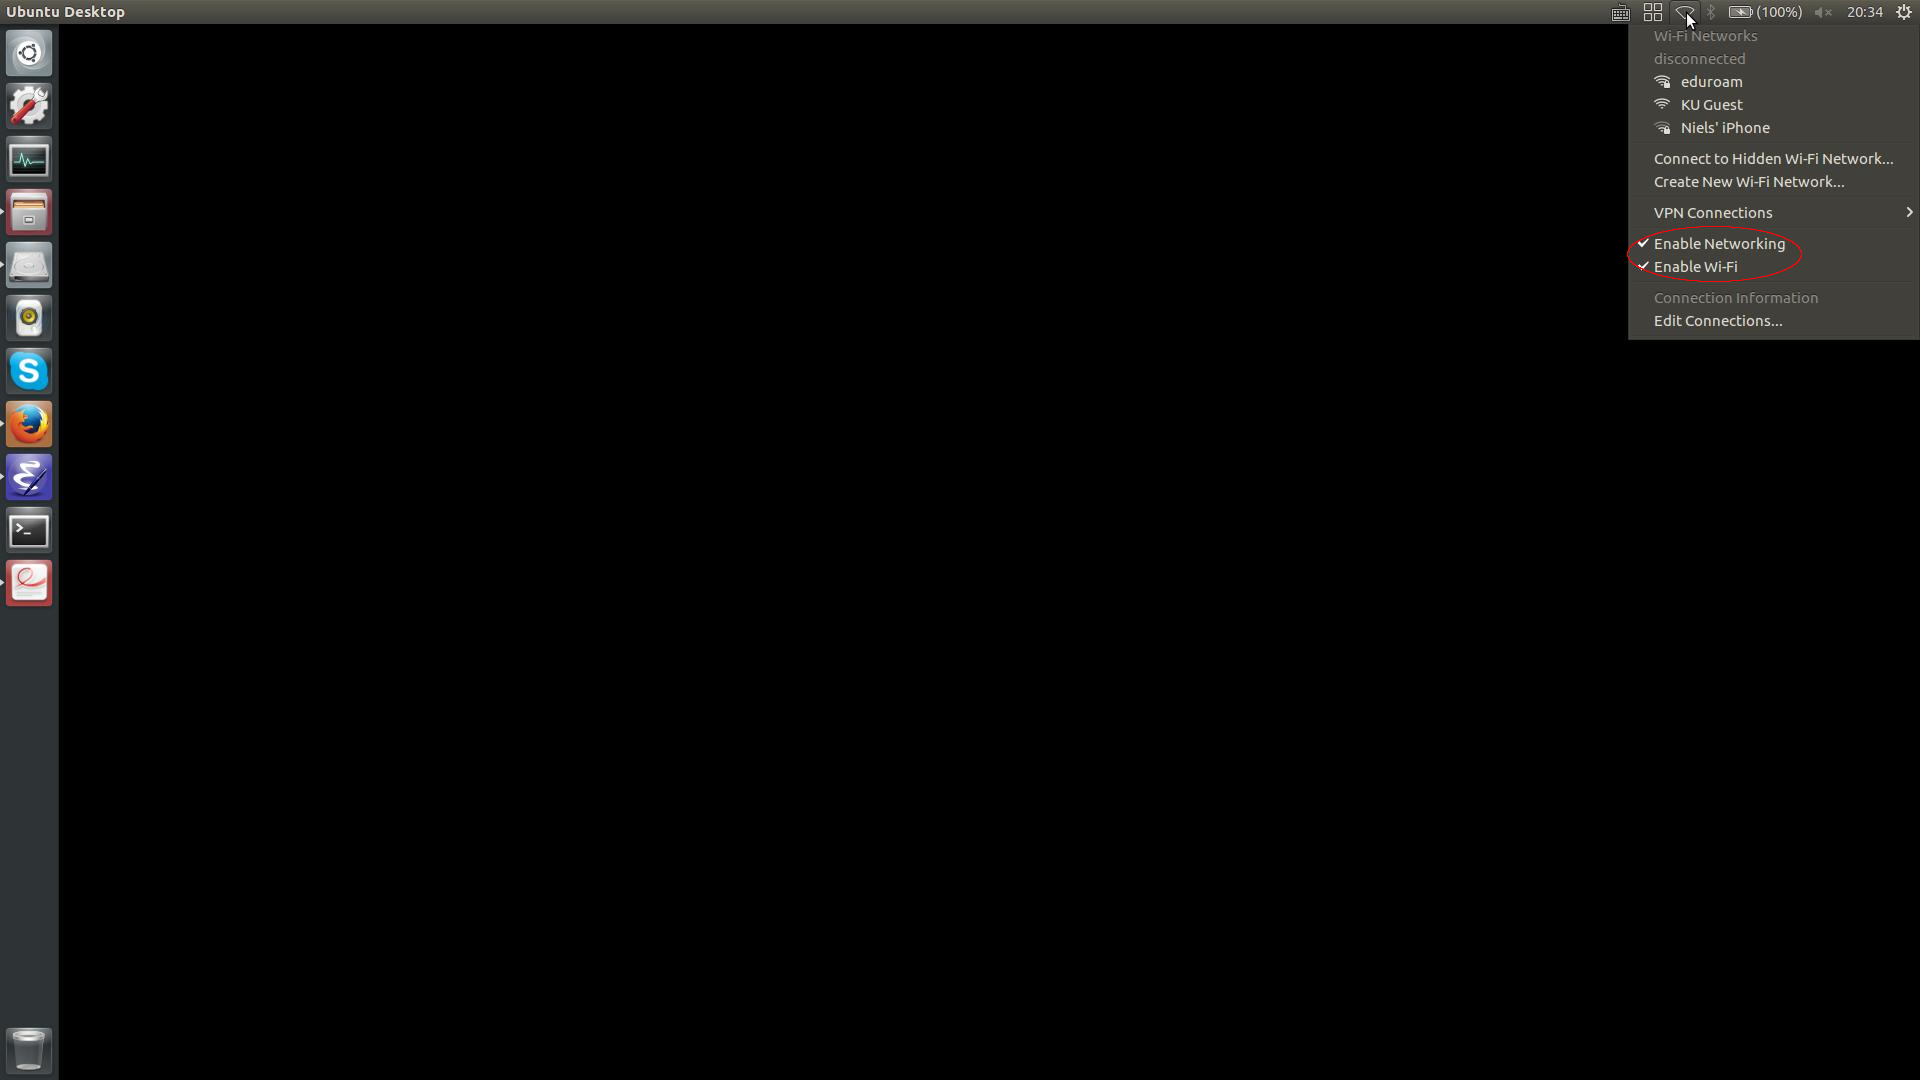
\includegraphics[width=0.8\textwidth]{pic1.jpg}
\end{figure}\\\\

\noindent
\textbf{Then choose the available network `` eduroam '', and a pop-up window shows like this:}
\begin{figure}[h!]
  \centering
  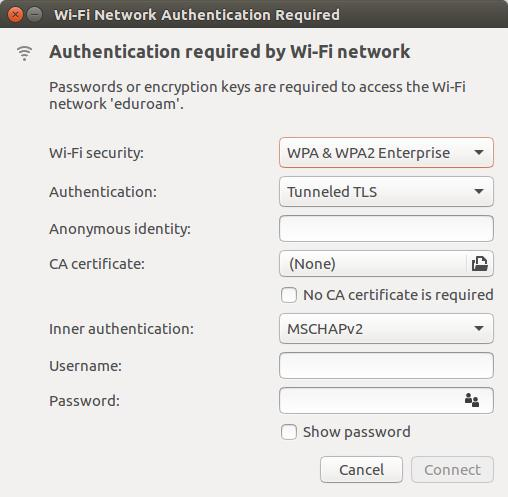
\includegraphics[width=0.4\textwidth]{pic2.jpg}
\end{figure}\\\\

\noindent
\textbf{We will first find the `` CA certificate '', which is called `` GeoTrust\_Global\_CA.pem ''. It's located in the `` /etc/ssl/certs '' folder.}\\
Click at `` None '' will open a window with your `` Home '' folder. You then need to go to your root folder (as screenshot below) to access the `` etc '' folder and so on.\\\\
OBS: Choose only `` GeoTrust\_Global\_CA.pem '', NOT `` GeoTrust\_Global\_CA\_2.pem '' !!
\begin{figure}[h!]
  \centering
  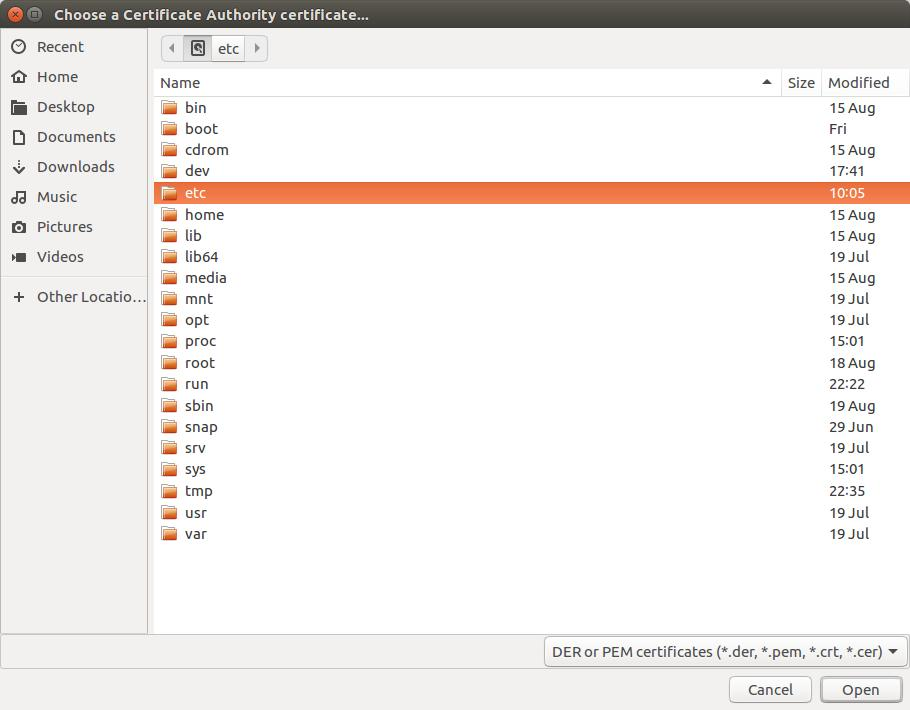
\includegraphics[width=0.7\textwidth]{pic3.jpg}
\end{figure}\\\\

\noindent
\textbf{Choosing the right certificate}\\
\begin{figure}[h!]
  \centering
  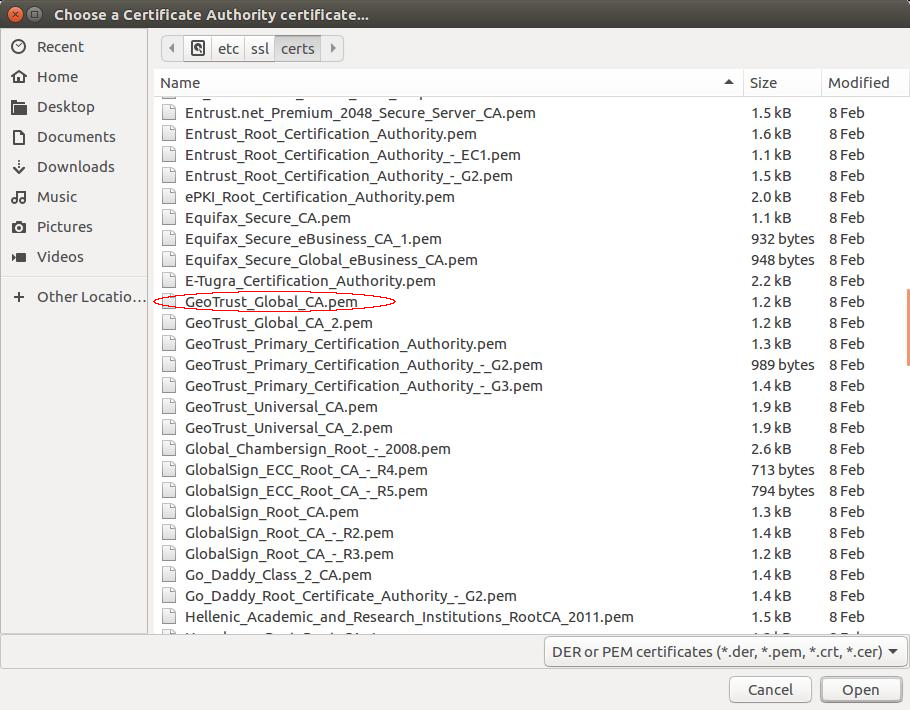
\includegraphics[width=0.7\textwidth]{pic3a.jpg}
\end{figure}\\\\


\noindent
\textbf{Now make sure you have select and filled the rows as below. If all set, the rows shall look like this:}\\
\textbf{(Note: if `` @ku.dk '' does not work for you, try `` @alumni.ku.dk '')}\\
\begin{figure}[h!]
  \centering
  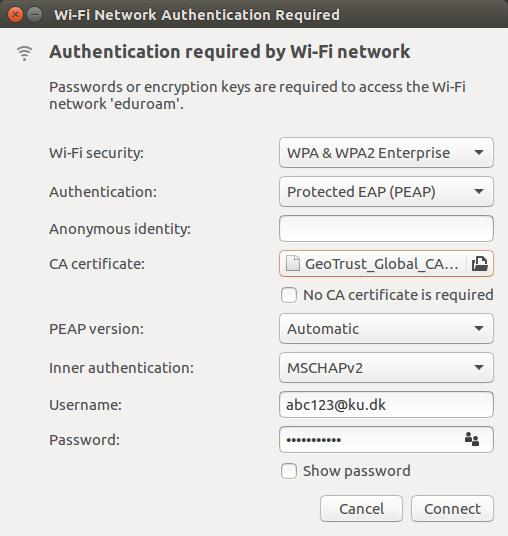
\includegraphics[width=0.4\textwidth]{pic4.jpg}
\end{figure}\\\\

\noindent
\textbf{Click `` Connect ''}

\end{document}

